\chapter{Technology}

\tocdata{toc}{$\rightarrow$\textit{Timon Koch}}
\section{Wombat}
\textbf{Author: Timon Koch}
The KIPR Wombat is the Controller currently used in the Botball competition. It consists of a raspberry pi 3b, a display and a casing, designed to include all necessery elements needed for the competition, such as ports for the various sensors, motors and servos allowed to be used and a cutout for the battery needed to power the used parts. Through the use of a raspberry pi 3b it is capable of wireless LAN and Bluetooth Low Energy. The Wombat uses the KISS (KIPR Instructional Software System) Web IDE developed by the KISS Institute for Practical Robotics. The current version supports ANSI C and can be used with a web browser and WiFi on any operating system.

\tocdata{toc}{$\rightarrow$\textit{Timon Koch}}
\section{Python}
\textbf{Author: Timon Koch}
Python is a powerful high-level, general purpose, object-oriented progrmming language with a design philosophy that emphasizes the readability of the written code through the use of significant indentation. 
It was created by Dutch programmer Guido van Rossum as a successor to ABC and was first released in 1991 with the capability of exepction handling. 
Features such as list comprehensions, reference counting, Unicode support and cycle-detecting garbage collections were introduced with Python 2.0 on 16 October 2000. After this release Python became a community-driven, open source project.
Due to a lack of backward compability, the switch from 2.7 to the 3.0 update, released in 2008, caused a big controversy. Folowing this most programs written in 2.7 had to be rewritten to support 3.0 update. 
Python has gained enormous popularity since the first release in the early 1990s and is used in a wide range of applications, ranging from web development to machine learning. 
The most important feature of the programming language Python is its support for mulitple programming paradigms, including object-oriented, imperative and functional programming. It was designed to be highly extensible via modules, rather than building all of itfunctionality into its core.

\tocdata{toc}{$\rightarrow$\textit{Maximilian Dragosits}}
\section{C++}
\textbf{Author: Maximilian Dragosits}

C++ is a precompiled programming language that combines low-level memory management with support for object-oriented, generic, and functional programming paradigms. 
It was designed by Danish computer scientist Bjarne Stroustrup with a focus on efficiency, performance, and flexibility.\footcite{lecture_essence_cpp} C++ has 
become widely used in various domains, including desktop applications, servers, video games, and digital equipment for space exploration.\\

It was standardized by the International Organization for Standardization (ISO) in 1998 as ISO/IEC 14882:1998 and has since evolved into a powerful programming 
language. The popularity of C++ has led to the creation of numerous libraries and frameworks, such as Catch2\footcite{catch2_git} and Doxygen\footcite{doxygen_main_site}. 
These frameworks are essential to the project's development and functionality.\\

C++ was chosen as one of the two frontend languages for this project due to its impressive speed and efficiency, as well as the vast ecosystem of external 
frameworks and libraries already available. The resources are essential in developing the RECT library, improving the project's capabilities and accelerating 
the development process. The decision to use C++ was a strategic choice, aligning with the language's strengths and the abundance of tools and resources it 
offers to the development landscape.

\tocdata{toc}{$\rightarrow$\textit{Jeremy Sztavinovszki}}
\section{Rust}
\addtocontents{toc}{\textit{Jeremy Sztavinovszki}\par}
\textbf{Author: Jeremy Sztavinovszki}

Rust is a general purpose multi paradigm programming language used in many fields ranging from embedded programming to web development. Although it is a relatively young language, having released its version 1.0 on May 15th 2015, it has seen great adoption from developers and has a big community. The language tries to be as fast as possibly, while still remaining memory-safe, which it achieves using its borrow checker. Even though it is possible to write unsafe code in Rust, that is not checked by the borrow checker, it is custom to keep the unsafe parts as small as possible.
Rust has a great ecosystem driven by the Rust Foundation and the Rust community. There are many tools, such as cargo, or rust-gdb, that provide great developer experience.
Right now there is now standardized async-runtime, so you normally use runtimes like tokio, async-std, or smol for programming asynchronously.

\tocdata{toc}{$\rightarrow$\textit{Christoph Fellner}}
\subsection{Cargo}
\textbf{Author: Christoph Fellner}

Cargo\footcite{cargo} is a build system and package manager for Rust, providing developers with a robust toolset for managing Rust projects. A rust package consists of a
\verb+Cargo.toml+ file, which contains metadata about the package, and a \verb+src+ folder, which contains the source code as rust-files (\verb+.rs+). It is an integral 
part of the Rust ecosystem and plays a crucial role in managing dependencies, building projects, and facilitating a smooth development workflow.

Here's an overview of Cargo's main functionalities:

\begin{itemize}
    \item 1. Dependency Management: Cargo manages project dependencies by automatically fetching and incorporating external libraries or crates. Developers specify 
        dependencies in the Cargo.toml file, and Cargo ensures the correct versions are used.
    \item 2. Project Structure: Cargo establishes conventions for organizing Rust projects, defining a standardized layout for directories and files. This consistency 
        helps developers understand and contribute to projects more easily.
    \item 3. Building and Compilation: Cargo handles the complexities of building and compiling Rust projects. Developers can use simple commands such as \verb+'cargo build'+ to 
        compile the code and \verb+'cargo run'+ to execute the compiled binary.
    \item 4. Testing: Cargo supports the integration of unit tests into Rust projects. Developers can use the \verb+'cargo test'+ command to run test suites, ensuring the 
        reliability and correctness of their code.
    \item 5. Documentation Generation: Cargo can generate documentation for Rust projects, making it easier for developers to create and maintain documentation for their 
        code. The \verb+'cargo doc'+ command generates and hosts documentation, and it can be published on platforms like \verb+docs.rs+.
    \item 6. Project Initialization: Cargo provides a convenient way to initialize new Rust projects with the \verb+'cargo new'+ command. This command sets up a new project with 
        the necessary directory structure and initial files.
    \item 7. Publishing: Cargo facilitates the process of publishing Rust packages (crates) to the official package registry, crates.io. This makes it straightforward for 
        developers to share their libraries and projects with the wider Rust community.
\end{itemize}

In essence, Cargo streamlines various aspects of Rust development, offering a standardized and efficient workflow for managing dependencies, building projects, testing 
code, generating documentation, and publishing packages. Its integration with the Rust toolchain contributes to the language's reputation for being developer-friendly and 
conducive to building robust and reliable systems.

\tocdata{toc}{$\rightarrow$\textit{Maximilian Dragosits}}
\section{gRPC}
\textbf{Author: Maximilian Dragosits}

gRPC\footcite{grpc_main_site} is an open-source framework that facilitates Remote Procedure Calls (RPC) across diverse environments. It is versatile 
and can be used in a broad spectrum of use cases, proving invaluable in establishing robust service-to-service connections. gRPC plays a pivotal role in the 
development of microservices and libraries. This framework is available in 11 different programming languages and provides developers with a flexible 
and accessible toolset for creating efficient and scalable communication channels.\\

gRPC's efficiency is central to its straightforward service definition and generation structure, which streamlines the integration process. 
This simplicity allows developers to focus on the core aspects of their projects, enhancing productivity and code maintainability. Furthermore, gRPC includes 
pluggable features such as authentication, load balancing, tracing, and health checking. These features provide developers with fine-grained control over 
service communication, ensuring robust and secure interactions within distributed systems.\\

In the context of the current project, gRPC plays a pivotal role. Its capability to seamlessly connect clients to backend services is particularly crucial. 
This feature enables efficient communication between Python and C++ frontends and the Rust backend, creating a cohesive and interoperable system. The project 
uses gRPC to achieve high communication efficiency, allowing for seamless data exchange between components and improving the overall performance and reliability 
of the system architecture.

\tocdata{toc}{$\rightarrow$\textit{Maximilian Dragosits}}
\section{Protocol Buffers}
\textbf{Author: Maximilian Dragosits}

Protocol Buffers offer a platform-neutral solution for serializing structured data, similar to formats such as XML, JSON, or YAML. They provide a versatile 
solution that seamlessly interfaces with automatically generated source code across an array of programming languages, catering to developers' preferences. 
Noteworthy among the supported languages are Java, Kotlin, Python, and various C-based languages, underscoring the broad applicability of Protocol Buffers 
in diverse development ecosystems.\\

Protocol Buffers enable developers to efficiently manage and exchange structured data across different platforms and systems. They provide a unified approach 
to serialization, whether using the robustness of Java, the conciseness of Kotlin, the flexibility of Python, or the performance advantages of C-based languages. 
This approach promotes interoperability, enabling developers to easily incorporate serialized data into their projects, thereby enhancing the efficiency and 
maintainability of their codebases.\\

An example of a Protocol Buffer file illustrates the elegance and conciseness inherent in this technology, demonstrating its role in facilitating efficient 
data interchange.

\begin{verbatim}
    syntax = "proto3";
    package msg;
    
    
    message From {
      string conn_name = 1;
      string topic = 2;
    }
    
    
    message To {
      string conn_name = 1;
      string topic = 2;
    }
    
    
    message Msg {
      bytes data = 1;
      oneof fromto {
        From f = 2;
        To t = 3;
      }
    }
\end{verbatim}

As can be seen in this example the first part of any .proto file is the definition of the protobuf language version. Either \textit{proto2} or \textit{proto3}. Next the package within this will be 
stored in when it is converted into a programming languages code is defined. In this case it will be \textit{msg}. After that you can import any other .proto file.
Then it is possible to define any amount of the following types and many others not used by this project:
\begin{enumerate}
    \item \textbf{message:} Defines a special data structure that houses multiple variables of potentialy different data types, which can then be used in other enums or services.
    \item \textbf{enum:} Defines an enum which acts like the equivalent type of structure in other programming languages. This can then be used in other parts of then .proto file.
    \item \textbf{service:} Defines a Remot Procedure Call (RPC) system. The generated code for this will include service interfaces and stubs to be used by RPC frameworks.
\end{enumerate}

\subsection{Protofile message definition}

Message types in proto3 are relatively simple to define.

\begin{verbatim}
    message message_name {
        field_type field_name = number;
      }
\end{verbatim}

First the \textit{message} keyword is used to signify that the following is a declaration for a message type. Then a freely choose able \textit{message\_name} is 
used as the name for the later resulting message structure. After that any number of fields can be defined within the curly brackets. The \textit{field\_type} can be
one of multiple supported data types, which includes but is not limited to double, flout, integer, boolean, string as well as bytes. After defining an appropriate
\textit{field\_name} this format requires the assignment of a number between 1 and 536,870,911 to each field in a message. This is required in order to identify
the field after encoding.

There are also three other modifiers, that can be applied to fields:

\begin{enumerate}
    \item \textbf{optional:} If a field with this modifier does not have its value explicitly set later it will instead return a default value. It also possible to check if this it has been set.
    \item \textbf{repeated:} A field with this modifier can be repeated any number of times within the message and the order of the repetition will be saved.
    \item \textbf{map:} A field with this modifier acts like a key/value pair with the definition syntax being like that of a C++ map.
\end{enumerate}

Another way of defining fields, that can have a multitude or a currently unkown type, is to use either the \textit{any} or the \textit{oneof} types.
The \textit{any} type is then later resolved by Protobufs internal reflection code.
\textit{Oneof} is then automatically later defined as one of the given data types within curly brackets placed after the \textit{field\_name} is given.

\subsection{Protofile enum definition}

Enums are share a lot of the same traits as message types in terms of the defintion syntax.

\begin{verbatim}
    enum enum_name {
        constant_value = number;
    }
\end{verbatim}

Similarly to messages the enum is given an \textit{enum\_name} and then any number of \textit{constant\_value}s can be defined. All of these constants need an associated
value in order to function properly and the first of those needs to have 0 as its number, so that the enum has a default value in cases like fields with the \textit{optional}
modifier. 
In order to bind multiple \textit{constant\_value}s to the same \textit{number} the \textit{allow\_alias} option must be set to true. This is done by inserting this line
into the enum before any definition of \textit{constant\_value}s:

\begin{verbatim}
    option allow_alias = true;
\end{verbatim}

Once an enum is defined then it can be used in other parts of the Protocol Buffer, as seen in this example:

\begin{verbatim}
    enum Success {
        Ok = 0;
    }

    enum SendError {
        NoSuchConnection = 0;
        SendFailed = 1;
    }

    message SendResponse {
        oneof result {
            Success s = 1;
            SendError err = 2;
        }
    }
\end{verbatim}

\subsection{Protofile service definition}

Services allow the easy generation of service interfaces and stubs to then be used by RPC implementations.

\begin{verbatim}
    service service_name{
        rpc rpc_name(message_type) returns (message_type) {}
        rpc rpc_name(message_type) returns (stream message_type) {}
    }
\end{verbatim}

A service is defined with a \textit{service\_name} and after that any number of inidvidual methods. In order to define the methods first the keyword \textit{rpc} must be used.
Then a name for the method is given through \textit{rpc\_name} and a parameter for the \textit{message\_type} that this method accepts. And then a \textit{message\_type}
is defined as the return value of the RPC. A stream of a particluar \textit{message\_type} can be defined by putting the keyword \textit{stream} before the type.

An example of this would be the SubListen service from this project:

\begin{verbatim}
    service SubListen{
        rpc listen(ListenRequest) returns (ListenResult) {}
        rpc subscribe(ListenRequest) returns (stream ListenResult) {}
    }
\end{verbatim}

\tocdata{toc}{$\rightarrow$\textit{Jeremy Sztavinovszki}}
\section{Nix}
\addtocontents{toc}{\textit{Jeremy Sztavinovszki}\par}
\textbf{Author: Jeremy Sztavinovszki}

Nix is one of a couple of things depending on the context. It is either a configuration language, a package manager, an operating system, or a build system.
That may seem a bit confusing, but the next section will cover each of these contexts for the sake of clearing up some of the confusion, that may arise from this statement.

\subsection{History}
Nix was first conceived and made a reality in 2003 as a research project by Eelco Dolstra. At first it was just a package manager, that could be run on any distro, but in 2007 it became its
own full blown Linux distribution with many other additions to the Nix eco system, such as Hydra \footcite{hydra}, a continuous intergration tool, and nixops,
a deployment tool for nixos deploying NixOS in a network/cloud \footcite{NixOps}. At the time of writing Nix has gotten another big addition in the form of flakes.
Flakes are a way of declaratively building anything ranging from Nix packages, over development environments, to system configurations. When a flake is build for the first time it
pulls in all of its inputs and writes their commit hashes to a flake.lock file. Through this mechanism of noting the exact commit each input of a flake it is possible to use nix flakes for
reproducible builds.

\subsection{The Language}
The language was the first part of Nix, that was implemented and it is arguably the most important part of Nix. Nix is a declarative functional programming language,
that is used for defining packages, build processes and configurations for a host of things ranging from reproducible development environments to IT-Infrastructure.
Taking an example for the syntax from the official nixos wiki site the language looks something like this:

% example here
\begin{minipage}{\textwidth}
\begin{lstlisting}[language=Nix, caption={Simple Examples of the Nix Language}]
#1
let
    a = 1;
    b = 2;
in a+b
# result 3

#2
let
    square = x: x*x;
    a = 12;
in square a
#result 144

#3
let 
    add = x: y: x+y;
in add 1 2

#result 3

#4
let
    square = {x ? 2}: x*x;
    a = 12;
in square{x=square {};}

#result 16
\end{lstlisting}
\end{minipage}

%description of the example here

In examining the provided code, a discernible pattern emerges. The syntax \newline \verb+let <variables> in <statement>+ serves as a method for defining values within a forthcoming block and it is quite reminicent of the Haskell programming language. However, this construct encompasses more than mere value assignment.
Consideration of each distinct block sheds light on its functionality. Block No. 1 initializes two variables, 'a' and 'b', then performs an addition operation on them. It's noteworthy that if an additional variable 'c' were defined but left unused, it would remain unevaluated due to Nix's lazy evaluation mechanism.
Moving to Block No. 2, it defines a function named 'square'. This function accepts a parameter 'x', as indicated by the notation \verb+x: x*x+. Parameter declarations in this context follow the structure \verb+<parameter name>: <statement>+. However, when multiple variables are required, as demonstrated in Block No. 3, the syntax adapts to \verb+<parameter name 1>:<parameter name 2>: <statement>+. This paradigm bears resemblance to lambda calculus \footcite{lambda_calculus}.
Block No. 4 showcases optional parameters. This feature is denoted by \newline \verb+{<parameter name> ? <default value>}: <statement>+.


\subsection{The Package Manager}
Nix, now a package manager, is a cross-platform package manager, that claims to have solved a problem called dependency hell \footcite{dependency_hell}, by keeping track of which package needs which dependencies. If a package is no longer needed it can automatically be garbage collected. Packages are installed to a directory called the nix store and have a unique hash, which is generated by combining some factors, like dependencies, versions and so on.
When defining a package you use the nix programming language and lazy functional programming to declare how to build it, what you need to build it and what files to install through a format called derivations.

\subsection{The Build System}
The following example showcases how to use the Nix language to define a flake containing a package, which can be built and installed on any system running the Nix package manager.
The specific example builds the latex files of which this thesis is comprised into a pdf file using a build tool called latexmk.
\medskip

\begin{minipage}{\textwidth}
\begin{lstlisting}[language=Nix, caption={The nix flake, that builds this diploma thesis}]
{
  description = "A flake to build the RECT-Diploma-Thesis";

  inputs = {
    nixpkgs.url ="github:nixos/nixpkgs/nixos-23.05";
  };

  outputs = {self, nixpkgs}:
  let
    system = "x86_64-linux";
    pkgs = nixpkgs.legacyPackages.${system};
  in {
		packages.${system}.default = pkgs.stdenv.mkDerivation rec {
			name = "RECT-Diploma-Thesis";

			src = ./.;

			buildInputs = [
				pkgs.texlive.combined.scheme-full
			];

			buildPhase = ''
					latexmk -pdf main.tex
			'';

			installPhase = '' 
					mkdir -p $out/pdf
					cp main.pdf $out/pdf
			'';
		};
  };
}
\end{lstlisting}
\end{minipage}

The code shown above is a nix flake. It defines the nixpkgs repository as an input and the result of the build process,
that is taking place in the mkDerivation block as an output. mkDerivation is a function which takes a name, pname, version, src,
buildInputs, buildPhase, installPhase, builder and shellHook as inputs and produces a package which is built in the standard environment (stdenv) \footcite{nixMkDerivation}.
The built derivation (or output of this flake) is then asigned a hash and stored in the nix store on the machine that built it.
An example of this would be the following path \newline\verb+/nix/store/dnx26izplgv46dwg548whh9kj5iz4vvx-RECT-Diploma-Thesis+. 

\subsubsection{Nixpkgs}
Of course the defined packages need to be stored somewhere. This is where the nixpkgs repository \footcite{nixpkgs_repo} on github comes in handy. It is a collection of over 80000 packages according to repology \footcite{repology_nixpkgs}.
The community can contribute their own definitions, or updates to the repository if they found something to be out of date, or missing. Of course when installing a package it is not built from scratch every time, like on source based distros.
Instead nixpkgs caches builds of the most popular packages, which then just have to be downloaded onto the users machines.

\subsection{The Operating System}
NixOS is built upon the Nix package manager. It is an independent Linux distribution, which means it is not based on any other Linux distribution like for example Debian, or Arch Linux.
What is really special about NixOS is, that the whole operating system with services, programs and all of the needed configurations can be built from one central file, which is written in the Nix Programming Language.
With this file stored as a backup a machine running NixOS could be up and running again in no time after a failure and through the usage of Nix Flakes it is possible to reinstall the system exactly the way it was before.

\tocdata{toc}{$\rightarrow$\textit{Jeremy Sztavinovszki}}
\section{Bluetooth Low Energy}
\addtocontents{toc}{\textit{Jeremy Sztavinovszki}\par}
\textbf{Author: Jeremy Sztavinovszki}
Bluetooth Low Energy (BLE) is a Low-Cost, Low-Bandwidth, Low-Energy technology, that works by transmitting data over the air using a slice of the frequencies available in the Industrial, Scientific and Medical Band \footcite{ism}.
It was introduced in the 4th version of the Bluetooth Version, after being developed by Nokia under the name Wibree and being adopted by the Bluetooth Special Interest Group (SIG). BLE at the time of its release made use of many
innovative technologies, for example Frequency Hopping Spread Spectrum \footcite{fhss}, which is used to avoid collisions when sending data. A combination of being innovative and marketing lead to BLE seeing a great adoption rate
after its initial release. Over the years Bluetooth Low Energy has seen many improvements, such as a Bluetooth Low Energy device being able to take on multiple roles simultaneously in the network.

\subsection{BLE Layers}
\subsubsection{Protocol vs. Profile}
The BLE specification has two important concepts, which it has clearly separated since its inception. These concepts are profiles and protocols. Hereby protocol is used to describe
the basic parts upon which the BLE stack builds and can be thought of the horizontal layers of the stack. Profile refers to vertical slices of the stack, that are used for specific use-cases when developing with BLE. Examples of a profile are.

\begin{itemize}
	\item The Glucose profile, which is used to securely transmit measurement data from e.g. insulin pumps.
	\item The Find Me profile, which allows devices to find one another
\end{itemize}

These use specific parts of the BLE protocol to achieve a specific task.

\subsubsection{Physical Layer PHY}
The Physical Layer (PHY) establishes the foundation for BLE communication by defining radio transmission properties such as modulation schemes, frequency bands, and power levels. It optimizes communication for BLE devices by employing techniques like frequency-hopping spread spectrum (FHSS) to mitigate interference and enhance reliability. Advancements in the PHY layer aim to improve data rates, extend range, and enhance spectral efficiency while maintaining low power consumption, which is crucial for the versatility of BLE applications.

\subsubsection{Link Layer (LL)}
The Link Layer(LL)
is responsible for managing essential functions such as connection establishment, maintenance, and data transmission between BLE devices. It handles advertising, scanning, and packet acknowledgment, optimizing power usage during data exchange. The efficient handling of packet formatting, acknowledgment, and error handling ensures a robust and reliable communication link, which is pivotal for BLE's energy-efficient operations.

\subsubsection{Host Controller Interface (HCI)}
The Host Controller Interface (HCI)
serves as the intermediary between the host (application processor) and Bluetooth hardware on the host side. It defines protocols and commands for seamless data exchange, enabling efficient control of Bluetooth functionalities.
The details of the host side are also included.

\paragraph{Host Side}
The HCI on the host side enables communication between the HCI driver and the application processor. It offers a standardised interface that defines the command structures and protocols used by the application to interact with the Bluetooth hardware. This abstraction allows for platform-independent communication and streamlines application development.
The Controller Side should also be considered.

\paragraph{Controller Side}
The HCI on the controller side translates commands from the host into hardware-specific operations for the Bluetooth controller. It facilitates communication between the host and the Bluetooth hardware, ensuring accurate execution of the required actions. This layer is responsible for managing data transfer between the host and controller, optimizing the transmission process


\subsubsection{Logical Link Controll and Adaptation Protocol (L2CAP)}
The Logical Link Control and Adaptation Protocol (L2CAP) efficiently multiplexes higher-layer protocols over BLE connections. It segments and reassembles data packets, optimizing data transmission efficiency while accommodating diverse application requirements. The role of protocol multiplexing and fragmentation is to ensure efficient data exchange while maintaining BLE's low-energy characteristics.

\subsubsection{Attribute Protocol and Generic Attribute Profile}
The Attribute Protocol (ATT) and Generic Attribute Profile (GATT) play critical roles in defining how data is exchanged and accessed between devices. ATT outlines rules for attribute information exchange, while GATT specifies the structure and mechanisms for accessing these attributes. The structured approach provided by data representation and interaction ensures interoperability across various applications and device types.

\subsubsection{Security Manager (SM)}
The Security Manager (SM) operates within the BLE protocol stack and is responsible for establishing secure connections and managing security-related aspects between BLE devices. It manages processes such as pairing, encryption, and authentication to ensure the confidentiality and integrity of data transmitted over BLE connections. This is critical for safeguarding sensitive information.

\subsubsection{General Access Profile}
The Generic Access Profile (GAP) is a fundamental layer in Bluetooth Low Energy (BLE) that is responsible for device discovery, connection setup, and addressing within the network. It defines device roles and manages how devices interact. GAP also handles device addressing, ensuring unique identification, and manages visibility, pairing, and power modes. GAP promotes interoperability between devices by standardizing essential functions. 
This ensures smooth communication across diverse BLE devices, regardless of their manufacturers or applications. The layer's importance lies in its ability to provide stability and reliability in BLE networks. GAP defines the following roles for a device to take on: 
\begin{itemize}
    \item{Broadcaster. The Broadcaster role is especially useful for applications, that regularily transmit data. It uses Advertising Packets instead of Connection Packets to send data in order for any listening device to be able to read the data without having to establish a conneciton.}
    \item{Observer. The Observer role is the counterpart to the Broadcaster. This role could be used for the base station of an alarm system, that receives broadcasts from sensors around the house for detecting intrusions.}
    \item{Central. The Central role is used to establish connections with peripheral devices. It always initiates the connections and is in essence the role, that allows devices onto the network. This is usually a smartphone and could be used for establishing a connection to some speakers to play music.}
    \item{Peripheral. The Peripheral role sends advertising packets in order for central devices to be able to find it and initiate connections.}
\end{itemize}

\subsection{Network Topologies}
Using the profiles described above, there is a wide range of network topologies that developers can choose from, depending on their objectives.
Some of the following topologies excel at saving power, while others are great for scalability and redundancy.

\subsubsection{Star Topology}
In a star topology, a central device (the 'Central') communicates with multiple peripheral devices. This configuration is similar to a hub-and-spoke model, where the central device manages and controls communication with the peripherals. For example, in a smart home scenario, a smartphone (acting as the central) connects to various peripherals such as smart locks, lights or sensors. The central device collects data from these peripherals and can also coordinate their functions. This architecture is simple and provides centralised control, but it relies heavily on the availability and range limitations of the central device.

\subsubsection{Mesh Topology}
BLE mesh networks allow devices to communicate with each other, forming a decentralised network without a central control point. Each device, or 'node', can communicate with nearby nodes, extending the coverage and redundancy of the network. For example, in a smart lighting system, each bulb can communicate with neighbouring bulbs to relay commands or data, ensuring robustness even if a node fails. Mesh networks are scalable, resilient and suitable for applications that require extensive coverage, such as smart buildings or large-scale sensor networks.

\subsubsection{Hub and Spoke Topology}
This architecture involves a central 'hub' device that communicates with multiple 'spoke' devices, each of which communicates only with the central hub. Think of a smart home setup where a central controller (e.g. a smart hub or gateway) manages and interacts with various sensors, smart appliances or actuators placed throughout the home. Each peripheral device communicates only with the central hub, streamlining communication and enabling centralised management.

\subsubsection{Cluster Tree Topology}
The cluster tree topology forms a hierarchical structure that organises devices into clusters, each cluster having a central node. These central nodes can communicate with other central nodes or higher level devices, creating a structured network. In industrial applications, devices within a particular area or zone can communicate with a local coordinator, which then communicates with higher level coordinators or a central system. This hierarchy enables efficient communication in large deployments, providing local and global control.

\subsubsection{Hybrid Architectures}
BLE applications often use hybrid architectures that combine multiple topologies to meet different needs. For example, a smart building might use a mesh network for inter-floor sensor communication, a star network for room-level control (with each room having a central controller), and a hub-and-spoke network for centralised management and integration of various systems within the building.

\tocdata{toc}{$\rightarrow$\textit{Timon Koch}}
\section{WiFi}
\textbf{Author: Timon Koch}

\subsection{History}
The history of WiFi, which stands for Wireless Fidelity, spans decades and involves numerous technological breakthroughs, standards developments, and the evolution of wireless communication. It is widely acknowledged that the story of WiFi begins with the quest for convenient and efficient wireless connectivity, driven by the ever-growing need for mobility and flexibility in computing and communication devices.

The origins of WiFi can be traced back to the late 19th and early 20th centuries, with the invention of radio waves and subsequent advancements in wireless communication technologies. Pioneers such as Nikola Tesla, Guglielmo Marconi, and Heinrich Hertz contributed significantly to the advancement of wireless communication principles.

During the 1970s, the concept of local area networks (LANs) became increasingly popular, particularly with the invention of Ethernet by Robert Metcalfe at Xerox PARC. Ethernet initially used coaxial cables and later switched to twisted pair wiring, which allowed computers to communicate within a limited physical area. This innovation laid the foundation for the eventual development of wireless LANs.

In the 1980s and 1990s, several wireless LAN protocols were developed, including proprietary ones like WaveLAN by NCR Corporation and the IEEE standard 802.11, which served as the foundation for WiFi. However, these early protocols had some limitations such as limited range, slow data rates, and interoperability issues.

The term 'WiFi' was coined in 1999 by the Wi-Fi Alliance, a non-profit organization established to promote wireless LAN technology and interoperability. The alliance included major technology companies such as Apple, Cisco, Nokia, and Symbol Technologies. In 1997, the IEEE released the first WiFi standard, IEEE 802.11, which provided a framework for wireless communication using radio frequencies.

 The IEEE 802.11 standard has undergone several amendments aimed at enhancing data rates, security, and reliability. Key milestones include 802.11a (1999), which operated in the 5 GHz frequency band and offered higher speeds than previous versions, and 802.11b (1999), which operated in the 2.4 GHz band and became widely adopted due to its compatibility with existing devices.

WiFi started to gain widespread adoption in the early 2000s, fueled by the proliferation of mobile devices, laptops, and the growing demand for wireless internet access in homes, businesses, and public spaces. The introduction of WiFi-enabled consumer electronics, such as smartphones, tablets, and smart TVs, further accelerated its adoption.

In recent years, there have been advancements in WiFi standards resulting in faster data rates and extended range. Standards such as 802.11n (2009) introduced multiple-input multiple-output (MIMO) technology, which significantly improved throughput and range. Subsequent standards such as 802.11ac (2013) and 802.11ax (Wi-Fi 6, 2019) have further enhanced speed, capacity, and efficiency.

WiFi has become an integral part of modern life, enabling wireless internet access in homes, offices, schools, airports, cafes, and public spaces worldwide. Its impact on how people work, communicate, and access information has been significant, driving digital transformation across various industries and sectors.

In the 2020s, WiFi 6E (802.11ax) emerged as the latest standard, introducing support for the 6 GHz frequency band, which significantly expands available spectrum and reduces congestion in wireless networks. As a result, it is expected to provide even higher data rates, lower latency, and better performance in dense deployment scenarios.

Looking ahead, the future of WiFi is likely to be shaped by advancements in technologies like Internet of Things (IoT), 5G integration, artificial intelligence (AI), and Wi-Fi 7 standards. These developments are anticipated to improve connectivity, security, and user experience in the increasingly interconnected world.

In conclusion, it can be said that the history of WiFi demonstrates remarkable human ingenuity and innovation in the pursuit of wireless connectivity. WiFi has transformed the way we connect, communicate, and interact with the world around us, from its humble beginnings as a nascent technology to its ubiquitous presence in today's digital age.

\subsection{Usage}
The use of WiFi has become widely adopted in modern society, transforming the way people connect to the internet, communicate, and interact with technology. WiFi provides wireless connectivity, allowing users to access the internet and network resources without the limitations of physical cables. Its usage spans various sectors and applications, greatly impacting daily life, business operations, and technological advancements.

WiFi is a widely used technology in consumer electronics, including smartphones, tablets, laptops, smart TVs, and smart home devices. These devices rely on WiFi to access the internet, stream media, download content, and communicate with other devices within a local network. In modern gadgets, WiFi has become an essential feature, providing users with the flexibility to stay connected and productive while on the go.

WiFi is considered essential for home networking, as it enables households to establish wireless internet connections for multiple devices simultaneously. WiFi routers and access points distribute internet connectivity wirelessly, allowing family members to browse the web, stream videos, play online games, and connect IoT devices without the hassle of wired connections. WiFi has become synonymous with home entertainment, productivity, and smart living, powering the connected homes of today.

Wireless connectivity is often considered a necessity in a variety of settings, such as offices, campuses, retail establishments, and public venues, particularly in the business world. WiFi networks can facilitate collaboration, communication, and productivity by enabling employees to access corporate resources, email, cloud services, and applications from anywhere within the premises. Enterprises utilise WiFi for a variety of purposes, including guest access, location-based services, asset tracking, and IoT deployments. This can lead to improved operational efficiency and enhanced customer experience.

 WiFi is frequently utilized in educational institutions, including schools, universities, libraries, and training centers. WiFi-enabled classrooms can enhance digital learning initiatives, online research, collaborative projects, and multimedia presentations. Both students and educators can benefit from wireless access to educational resources, e-books, online courses, and interactive learning platforms. The implementation of WiFi in educational settings has the potential to improve the educational experience by promoting connectivity, engagement, and innovation in learning environments.

 WiFi hotspots are frequently available in public areas such as airports, coffee shops, restaurants, hotels, malls, and transportation hubs. These locations offer WiFi access to customers, travelers, and visitors, enabling them to stay connected while on the go. This can improve customer satisfaction, loyalty, and time spent in commercial establishments, which can create opportunities for digital marketing, location-based services, and personalized experiences.

 WiFi technology plays an important role in healthcare settings, as it enables wireless communication, data exchange, and patient care delivery. Hospitals, clinics, and medical facilities use WiFi for electronic health records (EHR), telemedicine consultations, medical imaging, remote monitoring, and wearable devices. WiFi-enabled healthcare solutions can enhance efficiency, accessibility, and quality of care while ensuring compliance with privacy and security regulations.

The utilization of WiFi connectivity is considered to be of great importance for the widespread adoption of Internet of Things (IoT) devices, which serve a variety of purposes such as data transmission, control, and automation. WiFi networks are also utilized in smart homes, smart cities, and industrial IoT deployments to connect sensors, actuators, cameras, and devices for monitoring and management purposes. The integration of various IoT applications, such as home automation, energy management, traffic control, environmental monitoring, and infrastructure optimization, can be made possible through the use of WiFi.

WiFi enhances the entertainment and hospitality industry by providing seamless access to digital content, streaming services and interactive experiences. Hotels, resorts, theme parks and entertainment venues are deploying WiFi networks to provide guests with high-speed Internet access, in-room entertainment, mobile applications and concierge services. WiFi connectivity increases guest satisfaction, engagement and loyalty, driving revenue opportunities and brand differentiation in the competitive hospitality market.

In summary, the use of WiFi permeates every aspect of modern society, empowering individuals, businesses and communities with wireless connectivity, communication and innovation. As technology continues to evolve, WiFi will remain a critical enabler of connectivity-driven experiences, digital transformation and societal progress in the digital age.

\subsection{Function}

\subsection{Advancements}

\section{Libraries}

\tocdata{toc}{$\rightarrow$\textit{Maximilian Dragosits}}
\subsection{Catch2}
\textbf{Author: Maximilian Dragosits}

Catch2\footcite{catch2_git} is a unit testing framework specifically designed for C++. It seamlessly integrates with C++ code and offers a testing environment 
that aligns closely with the overall structure of C++ code. Its ability to harmonize with the natural syntax of functions and boolean expressions is noteworthy. 
Catch2 not only facilitates unit testing but also incorporates micro-benchmarking capabilities, enabling developers to analyze performance in detail.\\

In the context of our project, Catch2 is an ideal choice for shaping the C++ frontend. Its integration into the development process ensures that unit tests 
become an integral part of the codebase, fostering a culture of code reliability and maintainability. In addition, the integration of micro-benchmarking in Catch2 
is consistent with our project's objectives, enabling thorough performance evaluations. This feature is essential in promoting optimizations, as benchmarks provide 
valuable metrics for measuring the speed and efficiency of implemented methods.\\

By using Catch2, our project benefits from a versatile testing framework that not only validates the functionality of the C++ frontend but also enables developers 
to make informed decisions about enhancements and optimizations. Catch2's seamless integration and benchmarking capabilities make it a valuable asset in ensuring 
the robustness, performance, and efficiency of the implemented methods within the project.

\subsubsection{Unit Tests}

Unit Tests in Catch2 are defined very similarly as normal functions in C++. This example, pulled from the Github repository of Catch2, shows the simplicity of
this framework and its integration into projects.

\begin{verbatim}
    #include <catch2/catch_test_macros.hpp>

    #include <cstdint>
    
    uint32_t factorial( uint32_t number ) {
        return number <= 1 ? number : factorial(number-1) * number;
    }
    
    TEST_CASE( "Factorials are computed", "[factorial]" ) {
        REQUIRE( factorial( 1) == 1 );
        REQUIRE( factorial( 2) == 2 );
        REQUIRE( factorial( 3) == 6 );
        REQUIRE( factorial(10) == 3'628'800 );
    }
\end{verbatim}

First the relevant Catch2 headers are included and then a function with a return value is defined. In this case it is the function factorial. 
This function will be executed by Catch2 during the testing process. Then a test case is a macro defined as:

\begin{verbatim}
TEST_CASE(string testname, string tags) {...test...}
\end{verbatim}

The argument \textit{testname} is a arbitrary name given to the unit test, which is then later during the running of the test printed alongside the results of the macro.
Tags can be given to the test by inputting one or multiple tags into the \textit{tags} field and change the behavior of the macro accordingly. In the case of the example above
the only given tag is the name of the function to be tested. After this the \textit{TEST\_CASE} macro has a curly brackets-enclosed body in which the logic of the test can 
be defined.\\
This requires the use of other specific macros included in the Catch2 framework. For example:

\begin{verbatim}
REQUIRE( function(value) == expected_value );
CHECK( function(value) == expected_value );
\end{verbatim}

The two macros described above, REQUIRE and CHECK, operate in a similar way. They both execute the given \textit{function} with the provided \textit{value} or \textit{values}
and then assert if the returned data equals true or false according to the provided boolean operator. If it does then it was successful and the rest of the \textit{TEST\_CASE} is executed. The difference 
between REQUIRE and CHECK is however that if a REQUIRE macro fails it throws an exception and the unit test is stopped from executing the remainder of code inside it.

\subsubsection{Micro-benchmarks}
The benchmarking macros in Catch2 are defined similarly to how unit tests are. Benchmarking in itself is a useful practice, that provides a way to measure the performance
and speed of a particular function.

\begin{verbatim}
#include <catch2/catch_test_macros.hpp>
#include <catch2/benchmark/catch_benchmark.hpp>

#include <cstdint>

uint64_t fibonacci(uint64_t number) {
    return number < 2 ? number : fibonacci(number - 1) + fibonacci(number - 2);
}

TEST_CASE("Benchmark Fibonacci", "[!benchmark]") {
    REQUIRE(fibonacci(5) == 5);

    REQUIRE(fibonacci(20) == 6'765);
    BENCHMARK("fibonacci 20") {
        return fibonacci(20);
    };

    REQUIRE(fibonacci(25) == 75'025);
    BENCHMARK("fibonacci 25") {
        return fibonacci(25);
    };
}
\end{verbatim}

In the example above the unit test macros and benchmark macros from Catch2 are first included in order to be used later. The function to be benchmarked is then defined
After that the TEST\_CASE macro is used combined with the [\!benchmark] tag in order to turn this unit test into a benchmark. In the actual body of the test the function
is first tested weather or not it actually works as intended before any benchmarks are done. This is done with the REQUIRE macro, since it throws an exception if the 
assertion fails, preventing the rest of the benchmark from executing unnecessarily. If all the tests before the benchmarks pass then the actual BENCHMARK macros are
executed.

\begin{verbatim}
BENCHMARK(string name) {
    ... benchmark ...
};
\end{verbatim}

As part of the BENCHMARK macro a arbitrary name is given to it, which is then later during the output of the test used as a identifier for the specific benchmark.
Then the actual logic of the benchmark is then defined within curly brackets giving a lot of freedom in how a certain benchmark is executed. Adding a return statement
within the benchmark will ensure that the compiler doesn't mess with the test.\\
\vspace{\baselineskip}
After this is run a summary is automatically output within the command line window. This includes multiple data points that pertain to the execution speed of the tested
function:
\begin{enumerate}
    \item \textbf{Samples:} The amount of times the code within the curly brackets of the BENCHMARK macro is repeated in order to build a dataset to calculate the mean execution time.
    \item \textbf{Iterations:} The amount of iterations performed.
    \item \textbf{Estimated run time:} The estimated amount of time the code within the benchmark will take to run. Mesured in milliseconds.
    \item \textbf{Mean/low mean/high mean run time:} The mean time it will take for the code to run as well as the low mean and high mean for this in nanoseconds.
    \item \textbf{Standard deviation:} The standard deviation from the mean time in nanoseconds,
\end{enumerate}

\tocdata{toc}{$\rightarrow$\textit{Maximilian Dragosits}}
\subsection{Doxygen}
\textbf{Author: Maximilian Dragosits}

Doxygen\footcite{doxygen_main_site} is a versatile C++ framework that automates the generation of documentation for C++ code. It can also be used for other programming languages such as 
PHP, Java, Python, IDL, and Fortran. Doxygen extracts information directly from annotated source code, making the documentation process more efficient and 
accessible for developers.\\

Doxygen is notable for its flexibility in delivering documentation. The generated documentation can be accessed online through an HTML website or offline 
through a LaTeX document, providing options tailored to developers' preferences. Additionally, Doxygen can derive structure overviews even from non-annotated 
sources, facilitating a holistic understanding of the codebase. The project's architecture can be visualized more effectively by displaying entity relations 
through insightful graphs.\\

A quick overview of a Doxygen implementation shows a well-organized framework that streamlines the documentation process. This implementation improves code 
comprehension and promotes a collaborative development environment by providing a centralized repository of project documentation. The image shows how Doxygen's 
integration simplifies and enhances the documentation workflow, contributing to the clarity and accessibility of the project.\\

\begin{figure}[h]
	\centering
	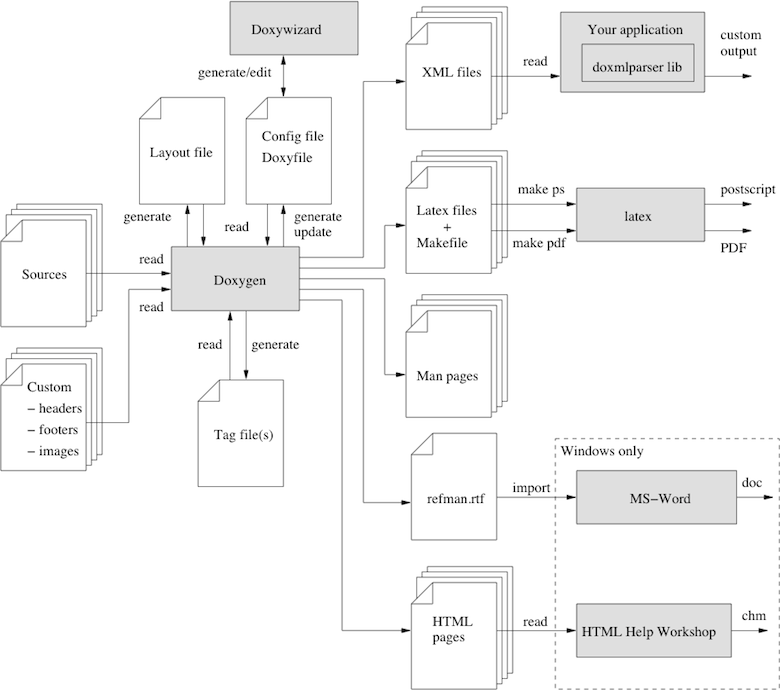
\includegraphics[width=\textwidth]{doxygenInfoflow.png} 
	\caption{Doxygen Infoflow diagramm\footcite{doxygen_main_site}}
	\label{pic:doxygenInfoflow}
\end{figure}

First a Doxygen config file, also called a \textit{Doxyfile} is generated in a project using the \textit{Doxywizard} and can be edited using this tool afterwards. 
This file is later read and updated during the generation process from \textit{Doxygen}. The layout files and tag files are also generated and used by \textit{Doxygen}
to facilitate the creation of the documentation.\\
\vspace{\baselineskip}
\textit{Sources} are the files with the actual source code, that will be part of the documentation, in them. These files are read alongside any other additional \textit{Custom}
files. For example the headers for source code, footers for the following document or images to be used in it. There are of course many other files that can be included
in order to refine the result further.\\
\vspace{\baselineskip}
Finally \textit{Doxygen} uses all this to generate documentation in the specified formats: XML, LaTex, Man, refman or HTML. \\

\subsubsection{Doxygen Configuration}
The first step in creating documentation with Doxygen is a configuration file. This can be automatically generated by the \textit{Doxywizard} with this command:

\begin{verbatim}
    doxygen -g <config-file>
\end{verbatim}

In this example \textit{<config-file>} is a stand-in for the name of the generated configuration file. There are many tags within this config file that change how 
the end result will look and what sources should be used or ignored. For example the INPUT tag specifies the location that \textit{Doxygen} will search for code and
EXCLUDE forbids it to use files contained within the given directories. After editing the file using a text editor or Doxywizard this command can be used to generate 
the documentation.

\begin{verbatim}
    doxygen <config-file>
\end{verbatim}

Doxygen normally requires the source code to be annotated in order to generate documentation, but a rough version can be made by setting the tag EXTRACT\_ALL to YES.
This will extract even the non-annotated classes and functions from the source code.

\subsubsection{Doxygen Annotation}

If the EXTRACT\_ALL tag is not enabled then the classes, functions and members within the source files need to be annotated in order to be picked up by \textit{Doxygen}
and turned into a documented section. There are many ways of signaling to \textit{Doxygen}, that you want it to produce documentation from a source. In general there
are two ways to do this:
\begin{enumerate}
    \item \textbf{Documentation within source:} In this way of annotation special comment blocks are inserted before and after parts of the source code. 
                This will cause the text within this special block to be displayed alongside the class, function, or member within the documentation.
    \item \textbf{Documentation outside source:} In this way of annotation the special comment blocks are written within a separate file and then connected 
                to the sources by way of a reference. With this method references to the source file need to be written within this distinct file.
\end{enumerate}

In \textit{Doxygen} special comment blocks are similar to C++ comments, but with extra characters in order to be picked up during generation. There are many different 
ways to define special comment blocks:\\
\vspace{\baselineskip}
\textbf{Javadoc and Qt style:} This way a special block can be definied just like a multi line comment in C++ with a special character after the first *.
\begin{quote}
\begin{verbatim}
    /**
     *   ... text ...
     */
\end{verbatim}
Or:
\begin{verbatim}
    /*!
     *   ... text ...
     */
\end{verbatim}
\end{quote}      
\vspace{\baselineskip}
\textbf{C++ comment style:} This style is similar to a C++ single line comment with an added / or ! at the begining.
\begin{quote}
\begin{verbatim}  
    ///
    ///  ... text ...
    ///
\end{verbatim}
Or:
\begin{verbatim}
    //!
    //!  ... text ...
    //!
\end{verbatim}
\end{quote}
\vspace{\baselineskip}
\textbf{Visible style:} This is a more clearly visible version of the previous two styles.
\begin{quote}
\begin{verbatim}
    /************************************
     *   ... text ...
    ************************************/
\end{verbatim}
Or:
\begin{verbatim}
    //////////////////////////////////////
    ///  ... text ...
    //////////////////////////////////////
\end{verbatim}
\end{quote}
\vspace{\baselineskip}

In documentation outside of the source additional commands are required. At the start of the document file a special comment block needs to have the name of the
file to be documented referenced by putting a backslash or an @ symbol before the filename in the first line of the block. After that any number of other 
special comment blocks can be defined with the first line in each of them being used to reference the desired class, function, member, struct, etc. This is done by
first using the equivalent structural commands and then inserting the definition statement of the chosen object. This can be seen in this example:\\

\begin{verbatim}
    /*! \fn int open(const char *pathname,int flags)
        \brief Opens a file descriptor.

        \param pathname The name of the descriptor.
        \param flags Opening flags.
    */
\end{verbatim}

In this case \textit{fn} is the structural command, which tells \textit{Doxygen} what type the object is.\\
\vspace{\baselineskip}

The other structural commands that can be seen in this example can be used in both documentation inside sources and outside sources. Using the \textit{brief} command 
is used to give a short description to the object and \textit{param} in order to signify and describe the parameters of this function.\\

\subsubsection{Doxygen Parsing}

During the documentation generation process, Doxygen parses special comment blocks and translates them into various output formats to create comprehensive 
documentation. The parser performs several key processes, culminating in the creation of documentation with Doxygen.

\begin{itemize}
    \item[] One of these processes is the conversion of Markdown writing within comment blocks into HTML, ensuring compatibility with web-based documentation platforms. This conversion improves the presentation of textual content, making it more accessible and visually appealing.
    \item[] Special commands embedded within the comment blocks are executed, allowing developers to include custom instructions or annotations. This feature empowers developers to tailor the documentation to specific project requirements, fostering flexibility and customization.
    \item[] Blank lines are handled appropriately. Paragraph separators are strategically used instead of blank lines to enhance the readability and organization of the generated documentation. This helps developers to better understand the information presented.
    \item[] Doxygen generates links to other sections of the documentation based on special comment blocks. The interlinking mechanism enables smooth navigation within the documentation, improving the user experience and promoting a cohesive understanding of the codebase.
    \item[] In situations where the output format is LaTeX, Doxygen converts HTML elements within the comment blocks into LaTeX commands. This transition ensures consistency and compatibility when generating LaTeX documents. It allows developers to choose the format that best suits their documentation needs.
\end{itemize}

\tocdata{toc}{$\rightarrow$\textit{Timon Koch}}
\subsection{Pytest}
\textbf{Author: Timon Koch}
Pytest is a testing framework for the Python programming language. It enables the creation of both simple unit tests and complex functional tests. Key features include test discovery, parameterized testing, and plugin support, making it a popular choice among Python developers. 
 
\subsubsection{Test Discovery}
The framework has the capability to automatically discover and execute test cases through a process known as 'test discovery'. By default, files that begin with 'test\_ ' or end with '\_test' are recognized as test files, although it is possible to explicitly mention other filenames. It is necessary for test method names to begin with 'test', as Test functions are identified by their names.
It is possible to either execute a specific test by indicating the corresponding identifier or execute all tests simultaneously. In the latter case, pytest will automatically detect and execute all files and functions that contain tests.  
By utilizing Pytest's plugin system, it becomes feasible to personalize and explore tests using supplementary mechanisms. The plugins available provide integration with diverse test frameworks, enabling the exclusion of particular tests or designating them for customized behaviors.

\subsubsection{Fixtures}
Fixtures are a useful feature that can help modularise and share setup code across multiple tests, resulting in improved code by increasing readability, maintainability and reusability.
They are defined as functions identified by the '@pytest.fixture' decorator. Different scopes may be specified to determine how long the fixture should last.

\subsubsection{Unit Tests}
Pytest provides compatibility with the 'unittest' testing framework. It is possible to discover and run both Pytest-style test functions and unittest test cases in the same project. This can facilitate a seamless transition between the two frameworks while leveraging the additional features provided by Pytest.

\tocdata{toc}{$\rightarrow$\textit{Christoph Fellner}}
\subsection{Rusqlite}
\textbf{Author: Christoph Fellner}

Rusqlite\footcite{rusqlite} emerges as a pivotal library, facilitating the seamless integration of SQLite capabilities into Rust code, akin to its analog, 
rust-postgres. This library provides a sophisticated interface, streamlining the execution of diverse database operations within the Rust programming paradigm. 
From the orchestration of table creation and data insertion to the intricacies of data querying, rusqlite empowers developers with a versatile toolset for 
database manipulation directly within their Rust codebase.

The decision to adopt rusqlite in our specific use case is underpinned by a meticulous consideration of three critical factors:

\begin{enumerate}
    \item \textbf{Portability:} SQLite's commendable attribute of cross-platform compatibility across diverse operating systems assumes paramount importance in 
    our context at RECT. Given the heterogeneous nature of small controllers operating within our system, the ability to seamlessly deploy SQLite databases 
    across different platforms becomes imperative for maintaining operational uniformity and efficiency.
    
    \item \textbf{Configuration:} In stark contrast to database systems that necessitate intricate setup procedures, SQLite obviates the need for complex 
    configurations. The simplicity inherent in working with SQLite aligns seamlessly with our operational requirements. The nominal requirement for a limited 
    number of tables further amplifies the pragmatic appeal of SQLite. In contrast to configuring a database on each controller, the minimal setup overhead 
    consolidates SQLite as the optimal choice for our streamlined operational demands.
    
    \item \textbf{Local:} SQLite distinguishes itself by eschewing the necessity for an external server or intricate installations. Its self-contained package 
    encapsulates all requisite features within a local environment. This intrinsic localization resonates with the operational ethos at RECT, aligning with the 
    need for an efficient and autonomous database solution without the encumbrance of external dependencies.
\end{enumerate}

In our specific instantiation, rusqlite is strategically employed for the persistent storage of the config.json file, a repository of vital data concerning 
available connections. The judicious selection of rusqlite in this context is grounded in its inherent advantages. The utilization of rusqlite markedly enhances 
the expediency and security of data access compared to traditional file-based retrieval mechanisms. This methodological choice contributes not only to the 
enhanced performance of our system but also underscores the commitment to preserving the integrity and reliability of configuration data, pivotal to the seamless
functionality of our application within the broader scientific and technological landscape.

\tocdata{toc}{$\rightarrow$\textit{Christoph Fellner}}
\subsection{Serde}
\textbf{Author: Christoph Fellner}

Serde\footcite{serde} emerges as a pivotal tool in the Rust programming ecosystem, dedicated to the efficient and generic serialization and deserialization 
(\textbf{ser}ialization/\textbf{de}serialization) of data structures. Offering a robust foundation for these operations, Serde plays a crucial role in optimizing
the handling of data structures within the Rust programming paradigm. For a comprehensive overview of Serde, interested readers can refer to the detailed 
documentation available at \href{https://serde.rs/}{https://serde.rs/}.\newline

The salient features of Serde become particularly evident in its capability to facilitate the seamless deserialization of JSON files with efficiency and 
simplicity. This functionality proves invaluable in our context, where the utilization of data from the config.json file is an integral part of our program. 
Serde streamlines this process, enabling us to incorporate the data effortlessly into our program with just a few lines of code.\newline

By leveraging Serde, we engage in a streamlined deserialization process wherein the data from the JSON file is efficiently transformed into a custom Rust 
structure. This bespoke structure, tailored to our specific needs, enables us to harness the deserialized data seamlessly within our program. The utilization of
Serde thus transcends mere deserialization, providing us with a powerful and adaptable mechanism to work with the data in a meaningful and efficient manner.\newline

In essence, the incorporation of Serde into our workflow is not merely a technical choice but a strategic one, driven by the need for optimized data handling 
and seamless integration of external data sources. Through Serde, our program gains a robust and flexible capability to decode JSON files, thereby enhancing the
overall efficiency and maintainability of our Rust-based application.

\tocdata{toc}{$\rightarrow$\textit{Christoph Fellner}}
\subsection{Tokio}
\textbf{Author: Christoph Fellner}

Tokio\footcite{tokio} serves as a pivotal asynchronous runtime for Rust, addressing the intricacies of asynchronous code execution in the language. In Rust, 
asynchronous code does not inherently execute independently; rather, it necessitates the use of a runtime like Tokio to effectively function. For an in-depth 
exploration of Tokio and its capabilities, readers are encouraged to delve into the detailed tutorial available at 
\href{https://tokio.rs/tokio/tutorial}{https://tokio.rs/tokio/tutorial}.\newline

The selection of Tokio as our asynchronous runtime is underpinned by several compelling reasons. Chief among them is Tokio's status as the preeminent and widely
adopted runtime for asynchronous Rust code. Its widespread usage within the Rust community attests to its robustness and reliability in facilitating asynchronous
programming paradigms.\newline

Moreover, Tokio's popularity is bolstered by the abundance of tutorials and educational resources available, making it approachable for developers seeking to 
harness the power of asynchronous programming in Rust. The simplicity and accessibility of Tokio's interface contribute to its widespread adoption, enabling 
developers to swiftly grasp and implement asynchronous patterns in their codebase.\newline

One of the key advantages of Tokio lies in its ability to execute multi-threaded asynchronous code safely. This capability is crucial in scenarios where 
parallelism and concurrency are essential, such as in web servers or applications handling numerous concurrent tasks. Tokio's adept handling of multi-threaded 
asynchronous code ensures the efficient execution of tasks without compromising safety or introducing race conditions.\newline


In summary, our decision to embrace Tokio as the asynchronous runtime for our Rust project is grounded in its status as the leading runtime in the Rust 
ecosystem, coupled with its user-friendly design and robust support for multi-threaded async code execution. This strategic choice positions us to harness the 
full potential of asynchronous programming in Rust, ensuring the responsiveness and scalability of our application.

\begin{verbatim}
#[tokio::test(flavor = "multi_thread", worker_threads = 2)]
async fn client_test(){ 
    let ser = test_server::run_server();
    println!("Server started");
    let cl = test_client::client_test();
    println!("Client started");

    tokio::select! {
        biased; 
        _ = ser => panic!("server returned first"),
        _ = cl => (),
    }           
}
\end{verbatim}

Using Tokio makes it possible to run multiple async functions at the same time. In the example above we start a server and a client and then wait for the first one to finish. 
This is done using the tokio::select! macro. The macro takes a list of futures and waits for the first one to finish. In our case we want to wait for the client to finish 
first, so we panic if the server finishes first. If the client finishes first we just return. Any occoring Errors are cathed and returned as Result.
The two functions \verb+run_server+ and \verb+client_test+ are both async functions. The server function is a simple echo server, that waits for a message from the client and 
then sends it back. The client function sends a message containing an url and a vote to the server and then waits for the response. Server and Client are connected via a gRPC 
connection. 

\tocdata{toc}{$\rightarrow$\textit{Christoph Fellner}}
\subsection{Tokio Rusqlite}
\textbf{Author: Christoph Fellner}

Tokio Rusqlite\footcite{tokiolite} stands as an innovative library at the intersection of Tokio and Rusqlite, synergizing their functionalities to enable 
asynchronous database interactions. This library represents a strategic amalgamation, providing developers with the capability to leverage Rusqlite seamlessly 
within an asynchronous programming paradigm facilitated by Tokio.\newline

The amalgamation of Tokio and Rusqlite in Tokio Rusqlite addresses the growing demand for asynchronous database operations in Rust. By integrating Tokio's 
asynchronous runtime with Rusqlite's capabilities, this library empowers developers to perform database operations without blocking the execution of other tasks.
This is particularly advantageous in scenarios where responsiveness and concurrency are paramount.\newline

Key features of Tokio Rusqlite include the ability to execute Rusqlite operations asynchronously, allowing for non-blocking interactions with SQLite databases. 
Asynchronous operations are vital in applications that require efficient handling of concurrent tasks, such as web servers, where multiple requests may be 
processed simultaneously.\newline

The seamless integration of Tokio Rusqlite into our development stack augments the versatility of Rusqlite by enabling asynchronous database operations. This is 
especially valuable in scenarios where responsiveness and scalability are critical factors. Leveraging Tokio Rusqlite in our project equips us with a robust 
solution for handling database interactions in an asynchronous manner, aligning with contemporary trends in Rust programming and distributed system 
architectures.

\tocdata{toc}{$\rightarrow$\textit{Christoph Fellner}}
\subsection{Tonic}
\textbf{Author: Christoph Fellner}

Tonic\footcite{tonic}, a Rust library that embodies the principles of gRPC, distinguishes itself with a keen focus on high performance, interoperability, and 
flexibility. Its seamless integration with the asynchronous paradigm, particularly its compatibility with Tokio, positions Tonic as a versatile tool for 
developing efficient and responsive distributed systems.\newline

The synergy between Tonic and Tokio is a noteworthy feature, as Tonic is crafted to align seamlessly with Tokio's asynchronous model. This compatibility not 
only enhances the performance of asynchronous Rust code but also simplifies the integration of Tonic into existing Tokio-based projects. Leveraging async/await 
functionality, Tonic facilitates a synchronous coding style in an asynchronous environment, making it a natural fit for projects utilizing Tokio.\newline

A distinctive aspect of Tonic lies in its support for gRPC, a high-performance remote procedure call (RPC) framework. Tonic employs Protocol Buffers to describe 
interfaces, providing a language-agnostic and efficient means of defining the structure of data. This approach not only enhances interoperability but also 
allows for the generation of necessary Rust code based on the defined Protocol Buffers, automating a significant portion of the development process.\newline

The utilization of Tonic in our project streamlines the definition of interfaces by leveraging Protocol Buffers. This enables us to articulate our interface 
specifications in a clear and concise manner, and Tonic then takes care of the Rust code generation, reducing manual effort and potential errors.\newline

In essence, Tonic serves as a powerful tool in our technology stack, providing a performant and flexible implementation of gRPC for Rust. Its compatibility with 
Tokio, support for async/await, and seamless integration with Protocol Buffers contribute to the development of robust and efficient distributed systems. By 
choosing Tonic, we aim to leverage its capabilities to enhance the performance, interoperability, and maintainability of our Rust-based projects.\newline

The example for Tokio above uses the Tonic library to convert the following Protocol-Buffer-file into Rust code, in order to use it in the client and server 
functions as Service.

\begin{verbatim}
syntax = "proto3";
package voting;
        
service Voting {
    rpc Vote (VotingRequest) returns (VotingResponse);
}
        
message VotingRequest {
    string url = 1;
        
    enum Vote {
        UP = 0;
        DOWN = 1;
    }
    Vote vote = 2;    
}
        
message VotingResponse {
    string confirmation = 1;
}
\end{verbatim}

In order to translate the Protocol Buffer into Rust code we use the \verb+include_proto!+ function from the Tonic library. This function takes the path to the 
Protocol-Buffer-file and generates the Rust code for the Service.

\tocdata{toc}{$\rightarrow$\textit{Christoph Fellner}}
\subsection{Docker}
\textbf{Author: Christoph Fellner}

Docker\footcite{docker} serves as an indispensable tool in modern software development, offering a containerization solution that facilitates the efficient 
execution of diverse applications within isolated environments known as containers. These containers, encapsulating applications and their dependencies, operate 
independently, enabling the concurrent execution of multiple containers on a single host system. The versatility of Docker extends from lightweight services 
like echo servers to complex web applications, making it a versatile choice for a spectrum of development and deployment scenarios.\newline

One of Docker's compelling use cases is the encapsulation of databases within containers. This capability enables the creation of portable and reproducible 
database environments, fostering ease of testing, development, and even benchmarking. In our specific use case, Docker proved instrumental in benchmarking 
different databases, allowing us to evaluate and identify the most suitable database for our application's requirements.\newline

Docker's open-source nature and compatibility across major operating systems contribute to its widespread adoption. Its availability on diverse platforms 
empowers developers to create consistent environments, irrespective of the underlying infrastructure. This feature is particularly advantageous in scenarios 
where multiple applications need to coexist on the same machine, as Docker mitigates compatibility concerns and ensures the isolation of applications from the 
local infrastructure.\newline

The ability to isolate applications from the host system's infrastructure is a key feature of Docker. This isolation not only enhances compatibility but also 
simplifies the deployment process. Developers can confidently run multiple applications on a single machine without the fear of conflicts or compatibility 
issues, streamlining the development and testing phases.\newline

In summary, Docker's role in our project extends beyond conventional application development and deployment; it serves as a pivotal tool for benchmarking 
databases. Its containerization approach, coupled with the ability to create reproducible environments, positions Docker as a valuable asset in our quest to 
identify the optimal database solution for our specific use case. The open-source nature and cross-platform compatibility further solidify Docker's standing as 
a cornerstone technology in contemporary software development and deployment practices.

\filbreak
